% !TEX TS-program = pdflatex
% !TEX encoding = UTF-8 Unicode

% This is a simple template for a LaTeX document using the "article" class.
% See "book", "report", "letter" for other types of document.

\documentclass[12pt]{book} % use larger type; default would be 10pt

\usepackage[utf8]{inputenc} % set input encoding (not needed with XeLaTeX)

%%% Examples of Article customizations
% These packages are optional, depending whether you want the features they provide.
% See the LaTeX Companion or other references for full information.

%%% PAGE DIMENSIONS
\usepackage[right=2cm,left=3cm,top=2cm,bottom=2cm,headsep=0cm,footskip=0.5cm]{geometry}
\usepackage{geometry} % to change the page dimensions
\geometry{a4paper} % or letterpaper (US) or a5paper or....
% \geometry{margin=2in} % for example, change the margins to 2 inches all round
% \geometry{landscape} % set up the page for landscape
%   read geometry.pdf for detailed page layout information

\usepackage{graphicx} % support the \includegraphics command and options

% \usepackage[parfill]{parskip} % Activate to begin paragraphs with an empty line rather than an indent

%%% PACKAGES
\usepackage{booktabs} % for much better looking tables
\usepackage{array} % for better arrays (eg matrices) in maths
%\usepackage{paralist} % very flexible & customisable lists (eg. enumerate/itemize, etc.)
\usepackage{verbatim} % adds environment for commenting out blocks of text & for better verbatim
\usepackage{subfig} % make it possible to include more than one captioned figure/table in a single float
% These packages are all incorporated in the memoir class to one degree or another...

%%% HEADERS & FOOTERS
\usepackage{fancyhdr} % This should be set AFTER setting up the page geometry
\pagestyle{fancy} % options: empty , plain , fancy
\renewcommand{\headrulewidth}{0pt} % customise the layout...
\lhead{}\chead{}\rhead{}
\lfoot{}\cfoot{\thepage}\rfoot{}

%%% SECTION TITLE APPEARANCE
\usepackage{sectsty}
\allsectionsfont{\sffamily\mdseries\upshape} % (See the fntguide.pdf for font help)
% (This matches ConTeXt defaults)

%%% ToC (table of contents) APPEARANCE
\usepackage[nottoc,notlof,notlot]{tocbibind} % Put the bibliography in the ToC
\usepackage[titles,subfigure]{tocloft} % Alter the style of the Table of Contents
\renewcommand{\cftsecfont}{\rmfamily\mdseries\upshape}
\renewcommand{\cftsecpagefont}{\rmfamily\mdseries\upshape} % No bold!

%%% Definiendo nuevos COLORES
\usepackage{xcolor} %Paquete de Color 
\definecolor{verde}{rgb}{0.25,0.5,0.35}
\definecolor{jpurple}{rgb}{0.5,0,0.35}

%%% Configurando el Layout para mostrar codigos Java
\usepackage{listings}
\lstset{
  language=Java,
  basicstyle=\ttfamily\small,
  keywordstyle=\color{jpurple}\bfseries,
  stringstyle=\color{red},
  commentstyle=\color{verde},
  morecomment=[s][\color{blue}]{/**}{*/},
  extendedchars=true,
  showspaces=false,
  showstringspaces=false,
  numbers=left,
  numberstyle=\tiny,
  breaklines=true,
  backgroundcolor=\color{cyan!10},
  breakautoindent=true,
  captionpos=b,
  xleftmargin=0pt,
  tabsize=4
}

%%% END Article customizations

\usepackage[spanish]{babel}
\usepackage{listings} 
\newcommand{\HRule}{\rule{\linewidth}{0.5mm}}
%%% The "real" document content comes below...


\title{Investigación del Lenguaje - Java}
\author{Adriana Rodríguez \and Marcelo Sánchez \and Raquel Villón Ramíez}

%\date{} % Activate to display a given date or no date (if empty),
         % otherwise the current date is printed 


\usepackage{eso-pic}
\newcommand\BackgroundEspol{
	\put(-218,338){
	\parbox[b][\paperheight]{\paperwidth}{%
           	\vfill
	           \centering
           	
\includegraphics[height=0.07\textheight,width=0.3\textwidth,keepaspectratio]{logoespol.jpg}%
	            \vfill
}}}

\newcommand\BackgroundFiec{
	\put(245,338){
	\parbox[b][\paperheight]{\paperwidth}{%
           	\vfill
	           \centering
           	
\includegraphics[height=0.07\textheight,width=0.22\textwidth,keepaspectratio]{logofiec.jpg}%
	            \vfill
}}}


\begin{document}


\begin{titlepage}
%\hspace*{0.2in}
\AddToShipoutPicture*{\BackgroundEspol}
\AddToShipoutPicture*{\BackgroundFiec}
%
\includegraphics[height=0.1\textheight]{logoespol}
%\hspace*{2.0in}
%
\includegraphics[width=0.3\textwidth]{logofiec}
%\includegraphics[width=0.1\textwidth]
\begin{center}
\textsc{\Large Escuela Superior Polit\'ecnica del Litoral}\\[1.0cm]
\textsc{\Large Facultad de Ingenieria en Electricidad y Computaci\'on}\\[1.5cm]

% Titulo
\HRule \\[0.4cm]
{ \LARGE \bfseries Investigaci\'on de Lenguajes - JAVA \\[0.4cm] }
\HRule \\[1.5cm]


% Autores
\begin{minipage}{0.4\textwidth}
\begin{flushleft} \large
\emph{Autores:}\\
Raquel \textsc{Vill\'on}\\
Adriana \textsc{Rodr\'iguez}\\
Marcelo \textsc{S\'anchez}
\end{flushleft}
\end{minipage}
\begin{minipage}{0.4\textwidth}
\begin{flushright} \large
\emph{Profesor:} \\
Ing.~Javier \textsc{Tibau}
\end{flushright}
\end{minipage}
\vfill
% Bottom of the page
{\large \today}
\end{center}
\end{titlepage}





%\maketitle
\tableofcontents

\newpage
\mbox{}

\chapter{Introducci\'on}
\paragraph{En este primer cap\'itulo se podr\'a analizar de acerca de qu\'e es Java, conocer acerca de las principales funcionalidades as\'i como tambi\'en las caracter\'isticas que destaca a este lenguaje orientado a objetos.}

\section{?`Qu\'e es Java?}

\paragraph{Java basicamente es un lenguaje compilador e interpretador \cite{ob} esto quiere decir que el c\'odigo que genera es revisado por una m\'aquina virtual (JVM) que lo que hace es mantener alejado el c\'odigo en bytecodes sin la necesidad de revisar que sistema operativo es la que contiene la m\'aquina en la que se est\'a trabajando. Adem\'as, la m\'aquina virtual ayuda con la gesti\'on de la memoria ya que este consta con la ayuda del recolector de basura (que mantiene un control de liberaci\'on de memoria) llevan un control din\'amico entre si.}

\paragraph{El recolector de basura (\textsl{Garbage Collector}) es el encargado principal del control de la localidad de la memoria para los objetos; dicho por \cite{sun} es el responsable que los objetos est\'en correctamente referenciados, siendo aquellos denominados como 'vivos' mientras que los objetos que no est\'an referenciados son considerados como objetos 'muertos' en lo que all\'i el recolector de basura se encarga de liberar el espacio de memoria que se hab\'ia establecido para ese objeto.}

\begin{center}
	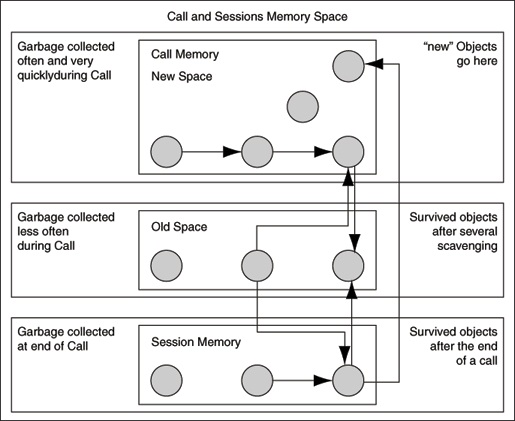
\includegraphics[scale=0.8]{garbage.jpg}
\end{center}
\paragraph{}

\chapter{Características}
\chapter{Historia}
\paragraph{Según los hermanos Deitel (2007), el lenguaje java fue creado en 1991 por la compañía Sun Microsystems, la cual es una empresa dedicada a la fabricación y venta de servidores y componentes de componentes informáticos. Empezó como un proyecto de investigación de la compañía denominado Green y fue pensado para programar los dispositivos electrónicos inteligentes.}
\paragraph{Deitel también indica que Java está basado en C++. Al principio su nombre fue Oak, pero luego se descubrió que ese nombre ya lo tenía otro lenguaje de programación. Luego, en una reunión de la gente de Sun en una cafetería, se propuso el nombre de Java, el cual es una variedad de café. }
\paragraph{Al principio el proyecto Green tuvo problemas debido a que el avance de los dispositivos electrónicos inteligentes no se desarrollaba tan rápido como Sun había previsto. Sin embargo, cuando la World Wide Web explotó, Sun vio rápidamente el potencial que Java tenía para darle dinamismo a las páginas web. De esa manera el proyecto Green pudo avanzar y finalizar con una conferencia en mayo de 1995, en la que Sun Microsystems anunció formalmente la existencia del lenguaje de programación Java. }
\paragraph{A medida que la World Wide Web avanzaba Java tenía mayor acogida y se desarrolló de tal modo en el que luego se lo utilizó para desarrollar grandes aplicaciones empresariales, aplicaciones para dispositivos móviles, radiolocalizadores, asistentes personales digitales, entre otros. }
\paragraph{En el 2009, Sun Microsystems fue comprada por Oracle por un valor de 7.400 millones de dólares según el portal 20minutos.es (2009) Y actualmente se distribuye la versión número 7 de Java, así como también sus diferentes líneas. Estas líneas se especializan en un ambiente, por ejemplo: Java SE está creada especialmente para aplicaciones de escritorio; Java EE es especializado en crear aplicaciones web; Java ME es utilizado para desarrollar aplicaciones que se ejecutan en dispositivos móviles, etc. }



\chapter{Tutorial de Instalación}
\paragraph{Para poder correr aplicaciones creadas en Java se necesita mínimo instalar Java Runtime Enviroment (JRE). Pero si lo que se quiere es desarrollar aplicaciones en Java, entonces necesita Java Development Kit (JDK) que contiene al JRE y herramientas para desarrollar, depurar y monitorear aplicaciones en Java (Oracle.com).}
\paragraph{En este documento mostraremos la instalación de Java SE 7, distribución para el desarrollo de aplicaciones de escritorio, en plataforma Windows 8 de 64bits. Para esto necesitaremos lo siguiente:}

\begin{enumerate}
\item Descargar el JDK directamente de la página oficial de Oracle. \\http://www.oracle.com/technetwork/java/javase/downloads/index.html.\\
Se muestra la opción para descargar sólo el JDK o el JDK con el IDE de desarrollo creado por Oracle, NetBeans. Escogeremos descargar sólo el JDK.
	
	\begin{figure}[h]
		\centering
			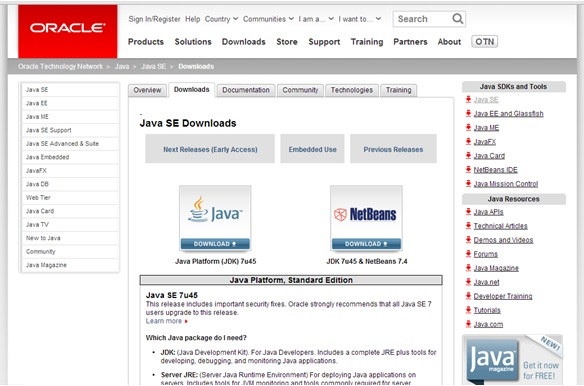
\includegraphics[width=10cm]{ins1.jpg}
			\caption{P\'agina de descarga del JDK.}
		
	\end{figure}
	
\item Para poder descargar el JDK debemos aceptar la licencia Y escoger el instalador adecuado para el Sistema operativo que se esté utilizando\\
\begin{center}
\begin{figure}[h]
		\centering
			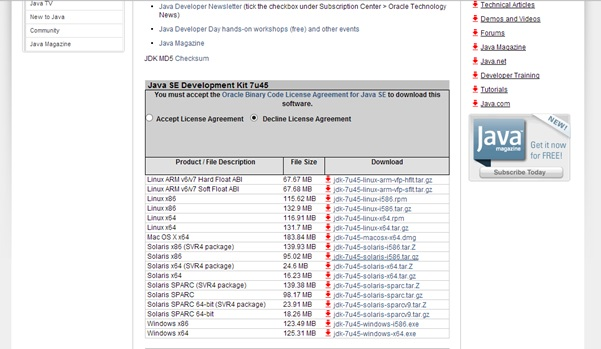
\includegraphics[width=10cm]{ins2.jpg}
			\caption{P\'agina de descarga del JDK.}
		
	\end{figure}
\end{center}
	
\item Preámbulo para escribir caracteres en español
\begin{figure}[h]
		\centering
			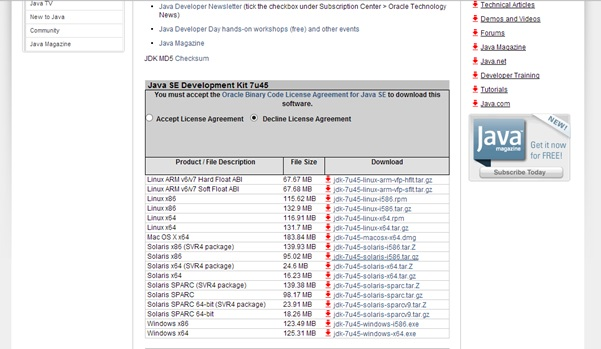
\includegraphics[width=10cm]{ins2.jpg}
			\caption{P\'agina de descarga del JDK.}
		
	\end{figure}
\end{enumerate}



\chapter{Hola Mundo y otros Programas Introductorios}

\paragraph{Cada vez que se usa una computadora, esta ejecuta múltiples aplicaciones que realizan tareas para el usuario. Los programadores, son los encargados de elaborar estas aplicaciones, escribiendo programas de cómputo que permiten a los usuarios cumplir sus tareas diarias.}
\paragraph{Ahora vamos a considerar una aplicación sencilla, la cual muestra únicamente una línea de texto, todo programador la ha elaborado en sus inicios.}
\noindent
\noindent
%
\begin{lstlisting}[frame=single]
/**
 * Este es un comentario
 */
 public class HolaMundo {
   public static void main (String argv[])
   {
     // Este tambien es un Comentario
     System.out.println("Hola mundo!");
   }
 }
\end{lstlisting}

\begin{thebibliography}{99}
\bibitem{ob} Belmonte, O. (2005). \textsl{Introducci\'on al lenguaje de programaci\'on Java}. [en l\'inea]. Disponible en: http://www3.uji.es/belfern/pdidoc/IX26/Documentos/introJava.pdf.

\bibitem{sun} Sun Microsystems. (2006). \textsl{Memory Management in the Java Virtual Machine} [en l\'inea]. Disponible en: http://www.oracle.com/technetwork/java/javase/memorymanagement-whitepaper-150215.pdf

\end{thebibliography}

\end{document}
